% 
% topic Template for ME3023 - Measurements in Mechanincal Systems - Tennessee Technological University
%
% Spring 2020 - Summer 2020
% Tristan Hill, May 31, 2020
% Module 3 - Calibration
% Topic 2 - The Calibration Curve   ->  (4th Topic)
%

%\documentclass{beamer}                         % for presentation (has nav buttons at bottom)
\documentclass[handout]{beamer}  % for handout 
\usepackage{beamerthemesplit}
\usepackage{amsmath}
\usepackage{listings}
\usepackage{multicol}
\usepackage{framed}

\beamertemplateballitem

\definecolor{TTUpurple}{rgb}{0.3098, 0.1607, 0.5176} % TTU Purple (primary)
\definecolor{TTUgold}{rgb}{1.0000, 0.8666, 0.0000} % TTU Gold (primary)

\setbeamercolor{palette primary}{bg=TTUpurple,fg=TTUgold}
\setbeamercolor{palette secondary}{bg=black,fg=TTUgold}
\setbeamercolor{palette tertiary}{bg=black,fg=TTUpurple}
\setbeamercolor{palette quaternary}{bg=TTUgold,fg=black}
\setbeamercolor{structure}{fg=TTUpurple} % itemize, enumerate, etc
\setbeamercolor{section in toc}{fg=TTUpurple} % TOC sections

% custom colors 
\definecolor{mygray}{rgb}{.6, .6, .6}
\definecolor{mypurple}{rgb}{0.6,0.1961,0.8}
\definecolor{mybrown}{rgb}{0.5451,0.2706,0.0745}
\definecolor{mygreen}{rgb}{0, .39, 0}
\definecolor{mypink}{rgb}{0.9960, 0, 0.9960}

% color commands
\newcommand{\R}{\color{red}}
\newcommand{\B}{\color{blue}}
\newcommand{\BR}{\color{mybrown}}
\newcommand{\K}{\color{black}}
\newcommand{\G}{\color{mygreen}}
\newcommand{\PR}{\color{mypurple}}
\newcommand{\PN}{\color{mypink}}
\newcommand{\GD}{\color{TTUgold}}
\newcommand{\OR}{\color{orange}}

\newcommand{\Lagr}{\mathcal{L}} % lagrangian

\newcommand{\hspcu}{\underline{\hspace{25mm}}} % large horizontal space w underline
\newcommand{\vspccc}{\vspace{6mm}\\} % large vertical space
\newcommand{\vspcc}{\vspace{4mm}\\}   % medium vertical space
\newcommand{\vspc}{\vspace{2mm}\\}     % small vertical space

\newcommand{\hspcccc}{\hspace{10mm}} % large horizontal space
\newcommand{\hspccc}{\hspace{6mm}} % large horizontal space
\newcommand{\hspcc}{\hspace{4mm}}   % medium horizontal space
\newcommand{\hspc}{\hspace{2mm}}     % small horizontal space


\author{ME3023 - Measurements in Mechanical Systems} % original formatting from Mike Renfro, September 21, 2004

\newcommand{\MNUM}{3\hspace{2mm}} % Module number
\newcommand{\TNUM}{2\hspace{2mm}} % Topic number  ->  (4th Topic)
\newcommand{\moduletitle}{Calibration }
\newcommand{\topictitle}{The Calibration Curve }

\newcommand{\sectiontitleI}{What is Calibration?}
\newcommand{\sectiontitleII}{Generalized Curve}
\newcommand{\sectiontitleIII}{Static Sensitivity and Zero Offet}
\newcommand{\sectiontitleIV}{Example: IR Distance Sensor}

\title{Module \MNUM - \moduletitle}

\date{Mechanical Engineering\vspc Tennessee Technological University}

\begin{document}

\lstset{language=MATLAB,basicstyle=\ttfamily\small,showstringspaces=false}

\frame{\titlepage \center\begin{framed}\Large \textbf{Topic \TNUM - \topictitle}\end{framed} \vspace{5mm}}

% Section 0: Outline
\frame{

\large \textbf{Topic \TNUM - \topictitle} \vspace{3mm}\\

\begin{itemize}
	\item \sectiontitleI		\vspc % Section I
	\item \sectiontitleII 	\vspc % Section II
	\item \sectiontitleIII 	\vspc %Section III
	\item \sectiontitleIV 	\vspc %Section IV
\end{itemize}

}

% Section I:
\section{\sectiontitleI}

\frame{
\frametitle{\sectiontitleI}

A \hspcu applies a known \hspcu to a measurement system for the purpose of observing the
system \hspcu. It establishes the relationship between the input and output values. The known
value used for the \hspcu is called the \hspcu. \vspc

\begin{itemize}
\item A range of input values can be used to form a calibration curve.
\item The calibration curve describes the input-output relationship of
the measurement system.
\end{itemize}

\vspace{10mm}
{\tiny Text: \underline{Theory and Design of Mechanical Measurements, 5th Edition}, }
}



% Section II:
\section{\sectiontitleII}

\frame{
\frametitle{\sectiontitleII}
\begin{multicols}{2}

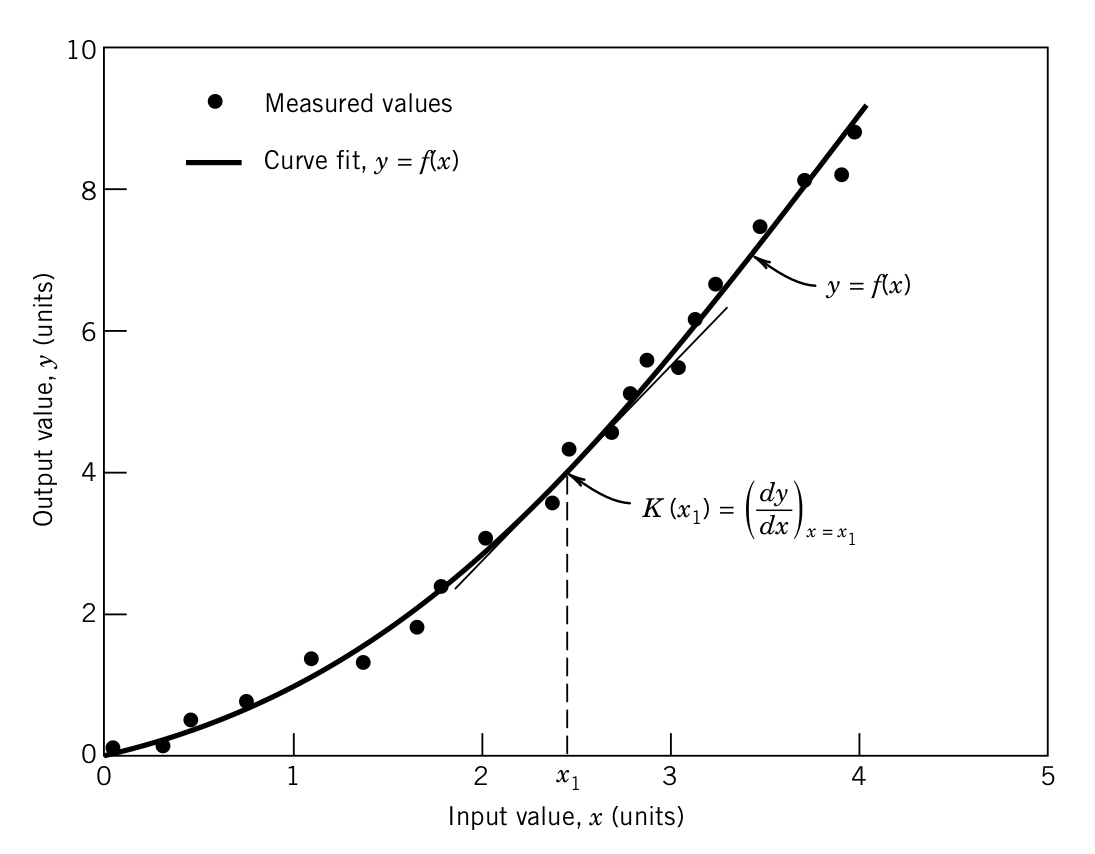
\includegraphics[scale=0.165]{calibration_curve.png}

\hspace{20mm} {\bf y}: measured signal\vspc 
\hspace{25mm} (output) \vspcc
\hspace{20mm} {\bf x}: known standard\vspc
\hspace{25mm} (input) \\
\end{multicols}

\textbf{Question:} How many values are needed for a calibration? Why?\vspc
{\tiny Image: \underline{Theory and Design of Mechanical Measurements, 5th Edition}, }
}

% Section III:
\section{\sectiontitleIII}

\frame{
\frametitle{\sectiontitleIII}

You have learned about these by a a different name. \vspcc

\hspcu - The Slope of the Calibration Curve \vspc

\hspcu - Y-Intercept of Calibration Curve \vspccc

\textbf{Question:} How many parameters or variables are needed to describe the curve?


}

% Section IV:
\section{\sectiontitleIV}

\frame{
\frametitle{\sectiontitleIV}

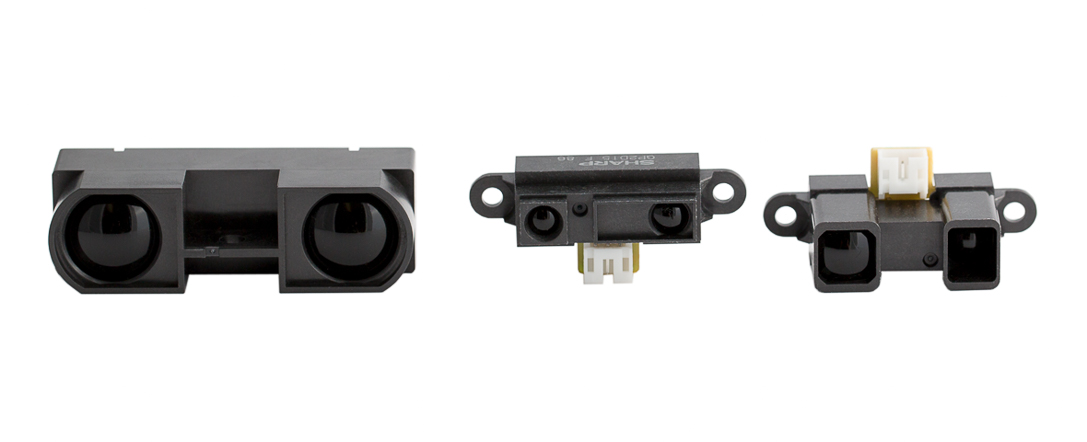
\includegraphics[scale=0.165]{sharp_ranger.jpg}

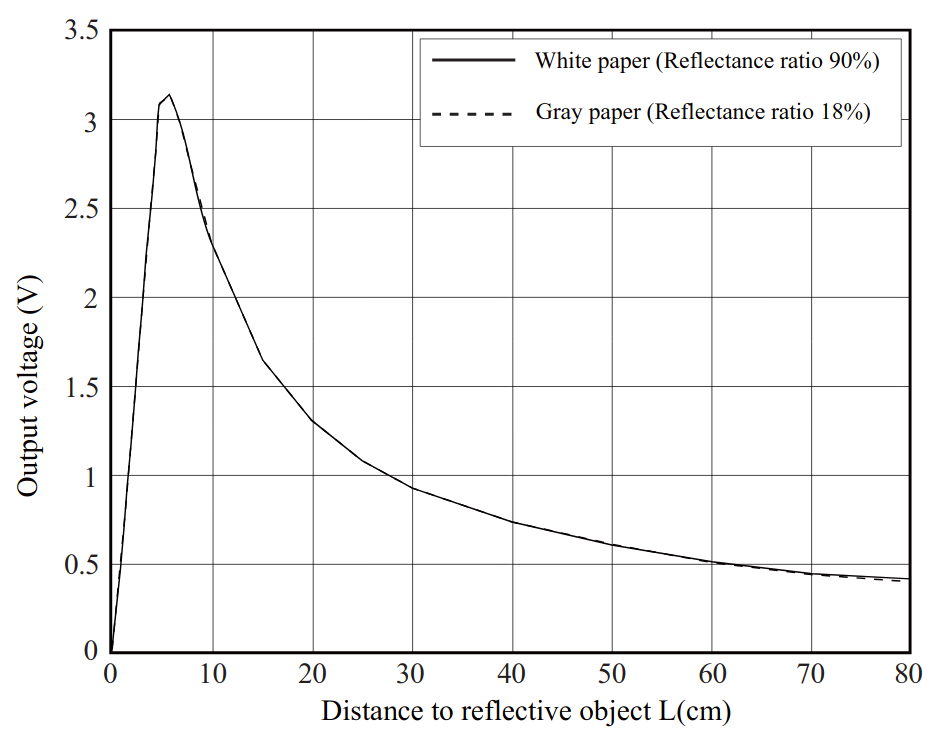
\includegraphics[scale=0.15]{sharp_calibration_fig1.png}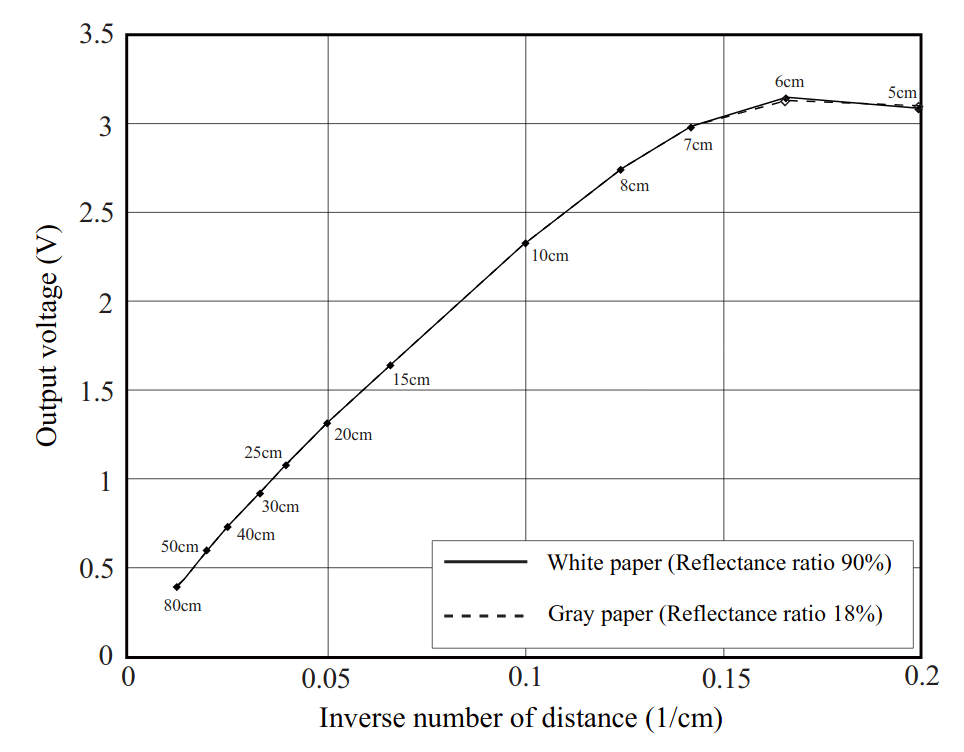
\includegraphics[scale=0.15]{sharp_calibration_fig2.png}
}


\end{document}






